\documentclass[a4paper]{article}
\usepackage{amsmath}
\usepackage{hyperref}
\usepackage{enumitem}
\usepackage{graphicx}
\usepackage[utf8]{inputenc}
\usepackage[T1]{fontenc}
\usepackage{textcomp}
\usepackage{gensymb}

\title{Master on Robotics: Perception Systems - Exercise 1.2}
\date{28-10-2015}
\author{Juan Pedro López Cabrera}

\begin{document}
  \pagenumbering{gobble}
  \maketitle

  \newpage
  \pagenumbering{arabic}

  \section{Exercise 2}
Go to the link: \url{http://www.hokuyo-aut.jp/02sensor/07scanner/utm_30ln.html}, which is a widely used lidar scanner in robotics.
\begin{enumerate}[label=\alph*.]
    \item Try to understand the specs by drawing them in a XY frame similar to the one of slide 11.

    \begin{figure}[ht]
      \centering
      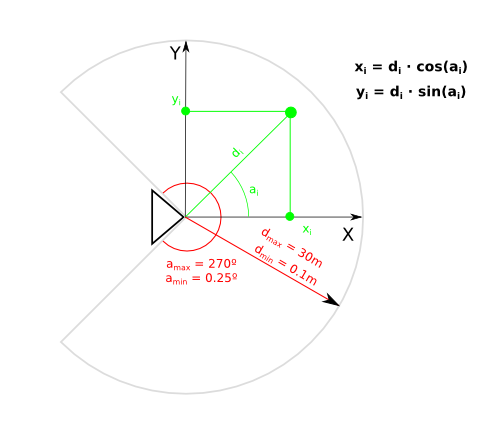
\includegraphics[scale=0.7]{Exercise_1_2_a}
      \caption{XY frame of UTM-30LN}
      \label{fig:xy_frame}
    \end{figure}

    \item which is the scan rate ?

If the scan time is 0.025s/scan, the scan rate is the inverse:

\begin{equation}
{scan\ rate} = \dfrac {1}{0.025} = {40}\ {Hz}
\end{equation}
    \newpage
    \item How many “laser hits” will get a pedestrian leg situated at 1m? and 3m? and 5m?. Draw a plot distance-hits. (make your own
assumption about pedestrian leg size)

We are going to assume a leg width of 0.15m (15cm) and the lidar specs indicate that the angular resolution is 0.25º. We want to find how many "slices" of 0.25º we can fit in a 0.15m wide leg depending on the distance from the lidar to the leg.
Here is the proposed formula:

\begin{equation}
{laser\ hits} = 1+\dfrac{\tan^{-1}(\dfrac{leg\ width}{distance})}{angular\ resolution}
\end{equation}

Given this equation, at 1m the leg will receive 35 hits of our lidar, at 3m it will receive about 12 hits and at 5m it will receive about 7.

\begin{figure}[ht]
  \centering
  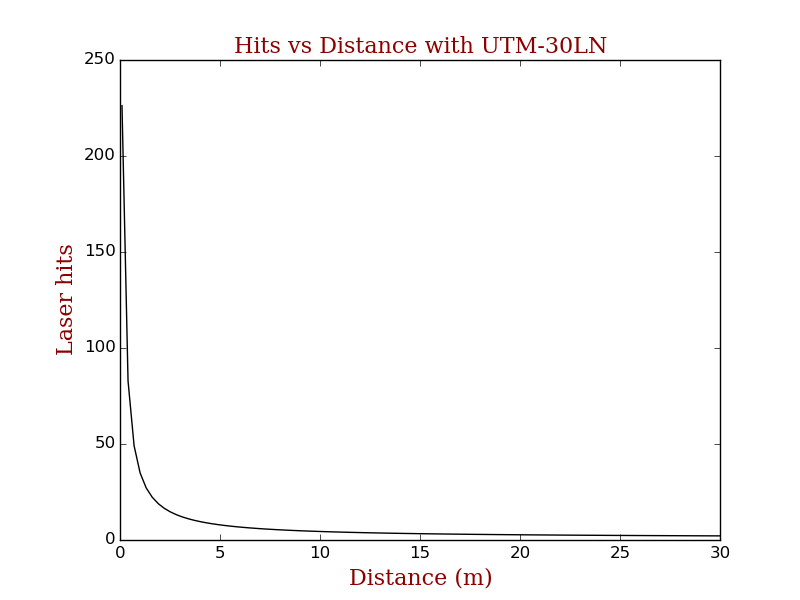
\includegraphics[scale=0.5]{Exercise_1_2_c}
  \caption{Distance vs Laser hits plot.}
  \label{fig:distance_laser_plot}
\end{figure}
\end{enumerate}

\end{document}
